\documentclass[11pt]{article}

\usepackage[margin=1in]{geometry}
\usepackage{lmodern}
\usepackage[T1]{fontenc}
\usepackage{microtype}
\usepackage{amsmath, amssymb, amsthm, mathtools, bm}
\usepackage{booktabs}
\usepackage{enumitem}
\usepackage{xcolor}
\usepackage{tikz}
\usepackage{float}
\usepackage{algorithm}
\usepackage{algpseudocode}
\usepackage[colorlinks=true, linkcolor=blue!50!black, citecolor=blue!50!black,
            urlcolor=blue!50!black]{hyperref}

\newtheorem{proposition}{Proposition}

\newcommand{\x}{\bm{x}}
\newcommand{\uu}{\bm{u}}
\newcommand{\vv}{\bm{v}}
\newcommand{\y}{\bm{y}}
\newcommand{\cc}{\bm{c}}
\newcommand{\grad}{\nabla}
\newcommand{\Op}{\bm{E}}
\newcommand{\nn}{\bm{n}}
\newcommand{\eps}{\bm{\varepsilon}}
\newcommand{\zz}{\bm{z}}
\newcommand{\E}{\mathbb{E}}
\newcommand{\N}{\mathcal{N}}
\newcommand{\Id}{\bm{I}}
\newcommand{\D}{D_\theta}
\newcommand{\ssb}{\sigma_{\mathrm{sb}}}

\title{I$^2$SB as posterior ascent with a bridge preconditioner}
\author{ImMAP project notes}
\date{November 2026}

\begin{document}
\maketitle

\noindent Diffusion samplers and bridge samplers do the same thing. Each runs an annealed
gradient ascent on a smoothed log-posterior, and a denoiser supplies the gradient. They differ
in how the network is shown its input. A very noisy state $\x_0+\sigma\eps$ is a poor network
input. A bridge re-expresses it as a bridge sample, which carries the same information but
stays bounded, so the network never sees large noise.
\begin{itemize}[leftmargin=1.5em, itemsep=1pt]
  \item Section~\ref{sec:ascent} states the ascent for any side information.
  \item Section~\ref{sec:bridge} introduces the bridge as a change of variables for the
        network input, and says why it helps.
  \item Section~\ref{sec:i2sb} derives I$^2$SB's sampler as this ascent~\cite{liu2023}, then
        maps it onto I$^2$SB's update line by line.
\end{itemize}

%=============================================================================================
\section{Posterior ascent}\label{sec:ascent}
%=============================================================================================

We want $\max_{\x_0}\log p(\x_0\mid\cc)$, where $\cc$ is the side information: a start image
$\x_1$, a measurement $\y$, or both. As in ImMAP~\cite{ks2021}, we ascend a Gaussian smoothing
of the objective while lowering the smoothing:
\[
  J_\sigma(\uu) \coloneqq \log p_\sigma(\uu\mid\cc),\qquad
  p_\sigma(\uu\mid\cc) = \int \N(\uu;\x,\sigma^2\Id)\,p(\x\mid\cc)\,d\x .
\]
So $J_\sigma$ is the log-density of the noisy target $\uu = \x_0+\sigma\eps$ given $\cc$, and it
tends to the objective as $\sigma\to0$. Its gradient is a denoiser (Tweedie):
\begin{equation}
  \sigma^2\grad J_\sigma(\uu) = D(\uu,\sigma;\cc) - \uu,
  \qquad D(\uu,\sigma;\cc) \coloneqq \E[\x_0\mid\uu,\cc].
  \label{eq:tweedie}
\end{equation}

\paragraph{The step.} Gradient ascent with step size $h\sigma^2$ is
\begin{equation}
  \uu^+ = \uu + h\sigma^2\grad J_\sigma(\uu) = (1-h)\,\uu + h\,D(\uu,\sigma;\cc).
  \label{eq:step}
\end{equation}
Tweedie's second-order identity gives
$-\grad^2 J_\sigma = (\sigma^2\Id - \operatorname{Cov}[\x_0\mid\uu,\cc])/\sigma^4
\preceq \sigma^{-2}\Id$. So every $h\in(0,2)$ increases $J_\sigma$, by the descent lemma.

\paragraph{The continuation.} After the step, fresh noise brings the iterate to the next,
smaller level $\sigma' = r\sigma$. An exact step leaves noise $(1-h)\sigma$, so the injection is
\begin{equation}
  \gamma^2 = \sigma'^2 - (1-h)^2\sigma^2 ,
  \qquad\text{which needs } h\in[1-r,\ 1+r].
  \label{eq:inject}
\end{equation}

\begin{algorithm}[H]
\caption{Annealed posterior ascent (\texttt{debiased\_ascent})}
\label{alg:ascent}
\begin{algorithmic}[1]
\Require denoiser $D(\cdot,\sigma;\cc)$; ladder $\sigma_N>\dots>\sigma_1>\sigma_0=0$ ($\sigma_N=\infty$
         allowed); steps $h_k\in[1-r_k,1]$ with $r_k=\sigma_{k-1}/\sigma_k$
\State $\uu_N \gets \sigma_N\zz$ \Comment{any $\uu_N$ if $\sigma_N=\infty$}
\For{$k = N,\dots,1$}
  \State $\vv_k \gets D(\uu_k,\sigma_k;\cc)$ \Comment{$=\uu_k + \sigma_k^2\grad J_{\sigma_k}(\uu_k)$}
  \State $\uu_{k-1} \gets (1-h_k)\,\uu_k + h_k\,\vv_k
         + \sqrt{\sigma_{k-1}^2 - (1-h_k)^2\sigma_k^2}\;\zz_k$
         \Comment{\eqref{eq:step}, \eqref{eq:inject}}
\EndFor
\State \Return $\uu_0$ \Comment{$=\vv_1$, since $\sigma_0=0$ forces $h_1=1$}
\end{algorithmic}
\end{algorithm}

\noindent Three step sizes are worth naming:
\begin{itemize}[leftmargin=1.5em, itemsep=1pt]
  \item $h = 1-r^2$ removes the variance $\sigma^2-\sigma'^2$ and injects
        $\gamma^2 = \sigma'^2(1-r^2)$. This is the VE ancestral sampler~\cite{song2021}.
  \item $h = 1-r$ injects nothing: the probability-flow ODE step.
  \item $h=1$ jumps to the estimate and re-noises it: SDEdit-style restarts~\cite{meng2022}.
\end{itemize}
At $\sigma_N=\infty$ we have $r=0$, so $h=1$ is forced. The first step then returns
$D(\cdot,\infty;\cc) = \E[\x_0\mid\cc]$, whatever $\uu_N$ is, and re-noises it to $\sigma_{N-1}$:
the ascent \emph{warm-starts itself} from the posterior mean.

%=============================================================================================
\section{Why a bridge}\label{sec:bridge}
%=============================================================================================

Algorithm~\ref{alg:ascent} needs the denoiser on the whole ladder, from very large (or infinite)
$\sigma$ down to $0$. At large $\sigma$ the input $\uu=\x_0+\sigma\eps$ is almost all noise:
\begin{itemize}[leftmargin=1.5em, itemsep=1pt]
  \item its norm grows like $\sigma$;
  \item the network must return $\approx\E[\x_0\mid\cc]$ while discarding all of it.
\end{itemize}
Standard diffusion copes in two ways. It rescales the input, as EDM's
$c_{\mathrm{in}}(\sigma)\uu$ does~\cite{karras2022}. And it stops at a finite $\sigma_{\max}$,
paying for the mismatch between $\N(\bm0,\sigma_{\max}^2\Id)$ and $p_{\sigma_{\max}}$.

When the side information contains an image $\x_1$ close to $\x_0$, there is a better
rescaling. Fix $V>0$ and feed the network
\begin{equation}
  \x_t = \x_1 + c(\sigma)\,(\uu-\x_1),\qquad c(\sigma) = \frac{V}{\sigma^2+V} = 1-t,
  \qquad t = \frac{\sigma^2}{\sigma^2+V}\in[0,1].
  \label{eq:x}
\end{equation}

\begin{proposition}\label{prop:bridge}
If $\uu=\x_0+\sigma\eps$, then $\x_t = (1-t)\,\x_0 + t\,\x_1 + \ssb(t)\,\eps$ with
$\ssb(t)^2 = Vt(1-t)$. This is the Brownian-bridge marginal from $\x_0$ to $\x_1$, with
$V=4\tau^2$. Conversely,
\begin{equation}
  \uu = \frac{\x_t - t\,\x_1}{1-t},\qquad \sigma^2 = \frac{Vt}{1-t}.
  \label{eq:u}
\end{equation}
For fixed $\x_1$ and $t<1$ the map is a bijection. So $\E[\x_0\mid\x_t,\x_1] =
\E[\x_0\mid\uu,\x_1]$: a regressor trained on bridge samples \emph{is} the denoiser that
Algorithm~\ref{alg:ascent} needs.
\end{proposition}
\begin{proof}
Substitute: $\x_1 + (1-t)(\x_0+\sigma\eps-\x_1) = (1-t)\x_0 + t\x_1 + (1-t)\sigma\eps$, and
$(1-t)^2\sigma^2 = (1-t)^2\,Vt/(1-t) = Vt(1-t)$.
\end{proof}

The level $\sigma = \ssb/(1-t) = \sqrt V\sqrt{t/(1-t)}$ is a standard deviation. It diverges as
$t\to1$, although $\ssb\to0$, because $\ssb$ vanishes only like $\sqrt{1-t}$. (The finite
quantity $\ssb^2/(1-t)=Vt$ is the variance of the forward process before it is pinned at $\x_1$.)

\paragraph{Why it conditions the problem better.} The bridge sample and the noisy target carry
the same information, but the bridge sample is the much better network input:
\begin{itemize}[leftmargin=1.5em, itemsep=1pt]
  \item \textbf{Bounded noise.} The noise the network sees, $c(\sigma)\sigma = \ssb(t)$,
        peaks at $\tau$ (at $t=\tfrac12$) and vanishes at both ends, while $\sigma$ runs from
        $0$ to $\infty$ (Figure~\ref{fig:ladder}).
  \item \textbf{Bounded signal, exact start.} The input stays near the segment from $\x_0$ to
        $\x_1$. At $\sigma=\infty$ it is exactly $\x_1$, a finite input the network is trained
        on. So the top of the ladder is $\sigma=\infty$ with no start mismatch, and the first
        step of Algorithm~\ref{alg:ascent} is the network's regression $\E[\x_0\mid\x_1]$.
  \item \textbf{A Wiener-filter preconditioner.} \eqref{eq:x} is $\E[\x_0\mid\uu]$ under the
        Gaussian prior $\x_0\sim\N(\x_1,V\Id)$. So the network is fed the linear-Gaussian
        denoiser's output, and an $\x_0$-predicting network learns only the correction. The
        better $\x_1$ predicts $\x_0$, the smaller that correction.
\end{itemize}
The bridge parameter $\tau$ encodes an assumed per-pixel spread $\sqrt V=2\tau$ of $\x_0-\x_1$.
It shapes the preconditioner and the ladder, but not the target: $\E[\x_0\mid\uu,\sigma,\x_1]$
does not depend on $V$. A guide of a different contrast fits the Gaussian assumption worse. That
makes the correction larger; it does not change what the network should learn.

\begin{figure}[H]
\centering
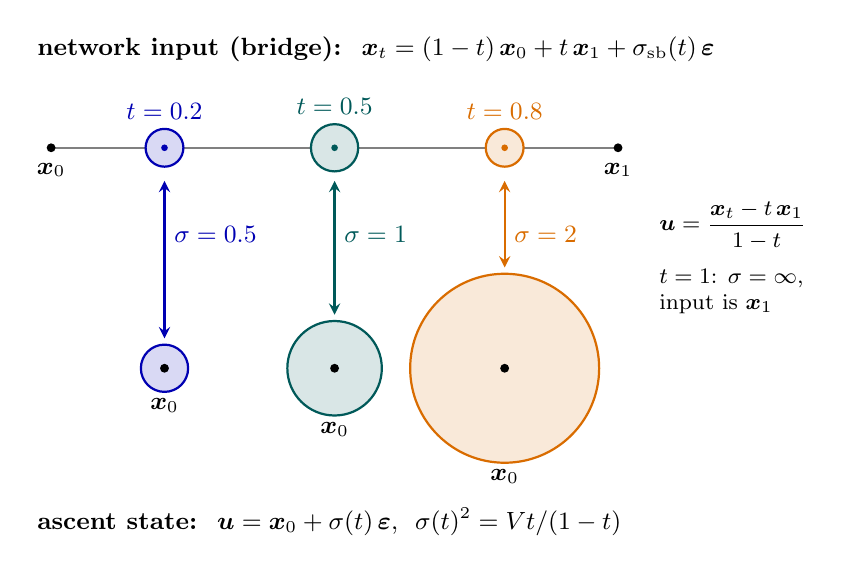
\begin{tikzpicture}[>=stealth, font=\small]
  \colorlet{ca}{blue!70!black}
  \colorlet{cb}{teal!70!black}
  \colorlet{cc}{orange!85!black}
  % ---- the bridge -----------------------------------------------------------------------
  \node[anchor=west] at (-0.3, 1.25) {\textbf{network input (bridge):} \
        $\x_t = (1-t)\,\x_0 + t\,\x_1 + \ssb(t)\,\eps$};
  \draw[gray, thick] (0,0) -- (7.2,0);
  \fill (0,0) circle (1.6pt) node[below=2pt] {$\x_0$};
  \fill (7.2,0) circle (1.6pt) node[below=2pt] {$\x_1$};
  \foreach \t/\r/\c in {0.2/0.24/ca, 0.5/0.30/cb, 0.8/0.24/cc} {
    \fill[\c!15] (7.2*\t, 0) circle (\r);
    \draw[\c, thick] (7.2*\t, 0) circle (\r);
    \fill[\c] (7.2*\t, 0) circle (1.2pt);
    \node[\c, above] at (7.2*\t, \r) {$t = \t$};
  }
  % ---- the denoising problems -----------------------------------------------------------
  \node[anchor=west] at (-0.3, -4.75) {\textbf{ascent state:} \
        $\uu = \x_0 + \sigma(t)\,\eps$, \ $\sigma(t)^2 = Vt/(1-t)$};
  \foreach \t/\r/\c/\s in {0.2/0.30/ca/0.5, 0.5/0.60/cb/1, 0.8/1.20/cc/2} {
    \fill[\c!15] (7.2*\t, -2.8) circle (\r);
    \draw[\c, thick] (7.2*\t, -2.8) circle (\r);
    \fill (7.2*\t, -2.8) circle (1.6pt);
    \node[below=-1pt] at (7.2*\t, -2.8 - \r) {$\x_0$};
    \draw[<->, \c, thick] (7.2*\t, -0.42) -- (7.2*\t, -2.8 + \r + 0.08);
  }
  \node[ca, right] at (1.44, -1.1) {$\sigma = 0.5$};
  \node[cb, right] at (3.60, -1.1) {$\sigma = 1$};
  \node[cc, right] at (5.76, -1.1) {$\sigma = 2$};
  \node[align=left, anchor=west, font=\footnotesize] at (7.6, -1.4)
        {$\uu = \dfrac{\x_t - t\,\x_1}{1-t}$\\[6pt]
         $t = 1$: $\sigma = \infty$,\\ input is $\x_1$};
\end{tikzpicture}
\caption{The same state in two coordinates. Bottom: the ascent state $\uu$, the target $\x_0$
plus noise $\sigma(t)$, which grows without bound toward $t=1$. Top: what the network is fed,
the bridge sample \eqref{eq:x}, whose noise $\ssb(t)$ stays below $\tau$ and vanishes at both
ends. The optimal outputs agree, $\E[\x_0\mid\x_t,\x_1] = \E[\x_0\mid\uu,\x_1]$. Radii drawn to
scale for $V=1$.}
\label{fig:ladder}
\end{figure}

\paragraph{Training.} The I$^2$SB loss $\E\|\D(\x_t,t,\x_1)-\x_0\|^2$, with
$t\sim\mathcal U[0,1]$, is conditional denoising with the preconditioner \eqref{eq:x}. In EDM's
vocabulary, only the design choices differ from a standard conditional diffusion:

\begin{center}
\small
\begin{tabular}{@{}lll@{}}
\toprule
 & conditional VE diffusion & bridge (I$^2$SB) \\
\midrule
ideal denoiser & $\E[\x_0\mid\uu,\sigma,\x_1]$ & the same \\
network input & $c_{\mathrm{in}}(\sigma)\,\uu$, e.g.\ $(\sigma^2+\sigma_{\mathrm{data}}^2)^{-1/2}\uu$
  & $\x_1 + c(\sigma)(\uu-\x_1)$ \\
training levels & e.g.\ log-normal $\sigma$ & $p(\sigma) = 2\sigma V/(\sigma^2+V)^2$ \\
top level & finite $\sigma_{\max}$, start $\N(\bm0,\sigma_{\max}^2\Id)$ & $\infty$, start $\x_1$ \\
sampling ladder & e.g.\ $\rho$-spaced in $\sigma$ & uniform in $t$ \\
\bottomrule
\end{tabular}
\end{center}

\noindent The identity needs a network that is given $\x_1$. Without \texttt{cond\_x1} (as in
I$^2$SB-Inversion) it learns $\E[\x_0\mid\x_t]$. That network reads $\x_1$ only through $\x_t$,
which works near $t=1$ but is not the conditional denoiser in general.

%=============================================================================================
\section{I\texorpdfstring{$^2$}{2}SB}\label{sec:i2sb}
%=============================================================================================

\subsection{The ascent I\texorpdfstring{$^2$}{2}SB runs}

Take Algorithm~\ref{alg:ascent} with $\cc=\x_1$ and three settings:
\begin{itemize}[leftmargin=1.5em, itemsep=1pt]
  \item the ladder $\sigma_k=\sigma(t_k)$ on a grid $1=t_N>\dots>t_0=0$, so $\sigma_N=\infty$;
  \item the ancestral step $h_k = 1-r_k^2$;
  \item the denoiser read through Proposition~\ref{prop:bridge},
        $D(\uu,\sigma;\x_1) = \D(\x_1 + c(\sigma)(\uu-\x_1),\,t(\sigma),\,\x_1)$.
\end{itemize}
Write $t=t_k$, $s=t_{k-1}$. By \eqref{eq:u}, $r^2 = \sigma_s^2/\sigma_t^2 = \frac{s(1-t)}{t(1-s)}$,
and the step is
\begin{equation}
  \uu_s = r^2\,\uu_t + (1-r^2)\,\vv + \sigma_s\sqrt{1-r^2}\;\zz,\qquad
  \vv = D(\uu_t,\sigma_t;\x_1).
  \label{eq:ustep}
\end{equation}

\subsection{Line by line into I\texorpdfstring{$^2$}{2}SB}

Map every state to the network's coordinates with \eqref{eq:x}, $\x_t = (1-t)\,\uu_t + t\,\x_1$:

\begin{center}
\small
\begin{tabular}{@{}lll@{}}
\toprule
line & ascent in $\uu$ (Algorithm~\ref{alg:ascent}) & I$^2$SB in $\x$ \\
\midrule
start & $\sigma_N=\infty$, $\uu_N$ arbitrary & $\x_{t_N} = \x_1$ \\
denoise & $\vv = D(\uu_t,\sigma_t;\x_1)$ & $\hat\x_0 = \D(\x_t,t,\x_1)$ \\
step & $\uu_s = r^2\uu_t + (1-r^2)\vv + \sigma_s\sqrt{1-r^2}\,\zz$
  & $\x_s = \tfrac st\x_t + \big(1-\tfrac st\big)\hat\x_0 + \sqrt{V\tfrac{s(t-s)}{t}}\,\zz$ \\
return & $\uu_0 = \vv$ at $\sigma_0=0$ & $\x_0 = \hat\x_0$ at $t_0=0$ \\
\bottomrule
\end{tabular}
\end{center}

\begin{proposition}\label{prop:lines}
Each row of the table is the same operation in two coordinates. The right column is I$^2$SB's
reverse step: the DDPM posterior of the bridge, $\x_s\sim\N\big(\tfrac st\x_t +
(1-\tfrac st)\hat\x_0,\ V\tfrac{s(t-s)}{t}\Id\big)$.
\end{proposition}
\begin{proof}
\emph{Start.} At $t=1$, $c=0$, so $\x_t=\x_1$ for every $\uu_N$.
\emph{Denoise.} $\x_t$ is the input \eqref{eq:x} of $\uu_t$, so $\vv=\hat\x_0$ by
Proposition~\ref{prop:bridge}.
\emph{Step.} Multiply \eqref{eq:ustep} by $1-s$ and add $s\x_1$. The coefficients are
\[
  (1-s)\,r^2 = \tfrac{s(1-t)}{t},\qquad (1-s)(1-r^2) = \tfrac{t-s}{t}.
\]
Substituting $\uu_t = (\x_t-t\x_1)/(1-t)$, the mean is
\[
  \tfrac st(\x_t - t\x_1) + \big(1-\tfrac st\big)\hat\x_0 + s\x_1
  = \tfrac st\x_t + \big(1-\tfrac st\big)\hat\x_0 .
\]
The noise variance is
\[
  (1-s)^2\sigma_s^2(1-r^2) = (1-s)^2\cdot\tfrac{Vs}{1-s}\cdot\tfrac{t-s}{t(1-s)}
  = V\tfrac{s(t-s)}{t}.
\]
\emph{Return.} At $t_0=0$, $\x=\uu$.
\end{proof}

\noindent For a general I$^2$SB schedule, replace $t$ by $m_n = \sigma_{\mathrm{fwd}}[n]^2/
\sigma_{\mathrm{fwd}}[N]^2$, and use $\sigma_n^2 = \sigma_{\mathrm{fwd}}[N]^2\,m_n/(1-m_n)$; the
proof is unchanged. \texttt{debiased\_ascent} (in \texttt{sb/i2sb\_recon.py}) implements the left
column. With I$^2$SB's step size and seed it reproduces \texttt{reverse\_sample} iterate for
iterate, to $2\cdot10^{-5}$ relative or better, with and without the CG step.

\subsection{What I\texorpdfstring{$^2$}{2}SB fixes, and what it frees}

\begin{itemize}[leftmargin=1.5em, itemsep=1pt]
  \item \textbf{The warm start is the first step.} With $\sigma_N=\infty$, the first update is
        $\uu_{t_{N-1}} = \E[\x_0\mid\x_1] + \sigma_{N-1}\zz$: regress, re-noise, then diffuse.
        This is the structure of SDEdit~\cite{meng2022} and come-closer-diffuse-faster
        \cite{chung2022}, with the initialisation from the network's own regression.
  \item \textbf{$\tau$ sets the noise scale.} On a fixed $t$-grid every $\sigma_k$ scales with
        $\sqrt V=2\tau$. At 20 uniform steps ($t_{N-1}=0.95$), $\sigma_{N-1}\approx1.7$ for
        $\tau=0.19$ and $\approx0.8$ for $\tau=0.09$, against image intensities $\sim1$.
  \item \textbf{The start image} (zero-filled, ACS, guide) changes only the conditioning and the
        centre of the preconditioner.
  \item \textbf{Freed by the $\uu$-form.} Algorithm~\ref{alg:ascent} accepts the same trained
        network with any step $h\in[1-r,1]$ (for example the deterministic $h=1-r$), any ladder,
        or a finite-$\sigma$ start from noise. I$^2$SB fixes $h=1-r^2$, the uniform $t$-grid and
        $\sigma_N=\infty$.
\end{itemize}

%=============================================================================================
\section{With a measurement: I\texorpdfstring{$^2$}{2}SB-Recon is ImMAP2}
%=============================================================================================

Adding a measurement $\y = \Op\x_0 + \nn$, with $\nn\sim\N(\bm0,\sigma_n^2\Id)$, to the side
information changes only the target, $\cc=(\x_1,\y)$. Since $\eps$ is independent of $\y$,
\eqref{eq:tweedie} still holds with $D = \E[\x_0\mid\uu,\x_1,\y]$. The network supplies
$\E[\x_0\mid\uu,\x_1]$. Approximating $p(\x_0\mid\uu,\x_1)\approx\N(\hat\x_0,\varsigma^2\Id)$
folds the data in:
\begin{equation}
  \bar\x_0 = (\Op^H\Op + \lambda\Id)^{-1}(\Op^H\y + \lambda\hat\x_0)
  \approx \E[\x_0\mid\uu,\x_1,\y], \qquad \lambda = \sigma_n^2/\varsigma^2 .
  \label{eq:prox}
\end{equation}
This is the CG step of I$^2$SB-Recon~\cite{wang2024}. ImMAP2 (\texttt{diffusion/immap.py}) runs,
at level $\sigma_k$: denoise to $\hat\x_0$, apply \eqref{eq:prox}, then
\begin{equation}
  \uu_{k+1} = \uu_k + h_k(\bar\x_0 - \uu_k)
  + \sigma_k\sqrt{(1-\beta h_k)^2 - (1-h_k)^2}\;\zz,
  \qquad \sigma_{k+1} = (1-\beta h_k)\,\sigma_k .
  \label{eq:immap2}
\end{equation}
Here $\sigma_{k+1}$ is the level the injection aims for; ImMAP2 then re-estimates it from the
next residual. This is Algorithm~\ref{alg:ascent} with $r = 1-\beta h$.

\begin{proposition}
With $r = \sigma_{k+1}/\sigma_k$, $h_k = 1-r^2$ and $\beta = 1/(1+r)$, the ImMAP2 step
\eqref{eq:immap2} is the I$^2$SB step \eqref{eq:ustep} with $\hat\x_0$ replaced by $\bar\x_0$.
That is I$^2$SB-Recon, written in the coordinates \eqref{eq:u}.
\end{proposition}
\begin{proof}
$1-\beta h_k = (1+r-1+r^2)/(1+r) = r$, so the next level is $\sigma_{k+1}$. The mean
$\uu_k + (1-r^2)(\bar\x_0-\uu_k)$ is that of \eqref{eq:ustep}, and the noise variance is
$\sigma_k^2(r^2 - r^4) = \sigma_{k+1}^2(1-r^2)$.
\end{proof}

So the two methods share the step structure exactly and differ only in its settings:

\begin{center}
\small
\begin{tabular}{@{}lll@{}}
\toprule
 & ImMAP2 & I$^2$SB-Recon \\
\midrule
denoiser & unconditional, prior $p(\x_0)$ & conditional, prior $p(\x_0\mid\x_1)$ \\
network input & $\uu$ & bridge sample \eqref{eq:x} \\
noise ladder & closed loop, $\sigma_k^2 = \tfrac1n\|\hat\x_0 - \uu_k\|^2$ & open loop, fixed
  $t$-grid \\
step size $h_k$ & schedule $h_0k/(1+h_0(k-1))$ & $1-r^2$, the variance removed \\
$\beta$ & fixed ($0.05$ by default) & $1/(1+r)$: $1$ on the first step, $\to\frac12$ \\
prox weight $\lambda$ & $\lambda_0\sigma_n^2(1+\sigma_k^2)/\sigma_k^2$ & constant
  ($7\cdot10^{-5}$) \\
start & noise at $\sigma_{\max}$, or a warm start & $\x_1$ at $\sigma=\infty$: regress, re-noise \\
\bottomrule
\end{tabular}
\end{center}

\noindent Modelling differs in the conditional prior and the bridge input; the rest are
schedules.
\begin{itemize}[leftmargin=1.5em, itemsep=1pt]
  \item \textbf{The prox weight.} ImMAP2's $\lambda_k$ is \eqref{eq:prox} with
        $\varsigma^2 = \sigma_k^2/(1+\sigma_k^2)$, the posterior variance under a unit-variance
        Gaussian prior, so it follows the noise level. A constant $\lambda$ assumes the denoiser
        is equally uncertain at every level.
  \item \textbf{The start decides what the prox contributes.} For the zero-filled start,
        $\x_1 = \Op^H\y$ is sufficient for $\y$, so $\E[\x_0\mid\uu,\x_1]$ already uses the data
        and \eqref{eq:prox} only corrects the network's errors. For a guide start,
        \eqref{eq:prox} is the only way $\y$ enters, as in ImMAP2.
\end{itemize}

%=============================================================================================
\section{Relation to standard diffusion}
%=============================================================================================

Since $\uu$ and $\x_1$ are independent given $\x_0$, Bayes' rule splits the conditional score,
and Tweedie turns the split into denoisers:
\begin{equation}
  \E[\x_0\mid\uu,\x_1] = \E[\x_0\mid\uu] + \sigma^2\,\grad_{\uu}\log p_\sigma(\x_1\mid\uu).
  \label{eq:bayes}
\end{equation}
So I$^2$SB is an unconditional VE diffusion plus a guidance term for $\x_1$. That term is
learned, where DPS~\cite{chung2023} approximates it through the denoiser's Jacobian.
\begin{itemize}[leftmargin=1.5em, itemsep=1pt]
  \item \textbf{Classifier-free guidance} would need the unconditional denoiser in the same
        $\uu$-coordinates. The bridge input depends on $\x_1$, so $D_\varnothing$ cannot share
        I$^2$SB's preconditioner.
  \item \textbf{A conditional-diffusion baseline} on the same $\x_1$ (SR3/Palette style) is not
        an independent method. It has the same target and the same sampler family, so any gap in
        results comes from the design choices of Section~\ref{sec:bridge}: above all, how well
        the network copes with its inputs at large $\sigma$.
\end{itemize}

\begin{thebibliography}{9}
\bibitem{liu2023}
G.-H.~Liu et al. I$^2$SB: Image-to-Image Schr\"odinger Bridge. \emph{ICML}, 2023.
\bibitem{ks2021}
Z.~Kadkhodaie, E.~P.~Simoncelli. Stochastic solutions for linear inverse problems using the
prior implicit in a denoiser. \emph{NeurIPS}, 2021.
\bibitem{song2021}
Y.~Song et al. Score-based generative modeling through stochastic differential equations.
\emph{ICLR}, 2021.
\bibitem{karras2022}
T.~Karras et al. Elucidating the design space of diffusion-based generative models.
\emph{NeurIPS}, 2022.
\bibitem{meng2022}
C.~Meng et al. SDEdit. \emph{ICLR}, 2022.
\bibitem{chung2022}
H.~Chung, B.~Sim, J.~C.~Ye. Come-closer-diffuse-faster. \emph{CVPR}, 2022.
\bibitem{wang2024}
Y.~Wang et al. Guided MRI reconstruction via Schr\"odinger bridge. arXiv:2411.14269, 2024.
\bibitem{chung2023}
H.~Chung et al. Diffusion posterior sampling for general noisy inverse problems.
\emph{ICLR}, 2023.
\end{thebibliography}

\end{document}
